
\documentclass[runningheads]{llncs}
\usepackage{graphicx}
\usepackage{apacite}
\usepackage{float}
\usepackage{listings}
\begin{document}

\title{Programming Assignment 1}
\subtitle{Designing a web crawler}

\author{
  Jaka Kokošar
  \and
  Danijel Maraž
  \and
  Toni Kocjan
}


\institute{Fakulteta za Računalništvo in Informatiko UL
\email{dm9929@student.uni-lj.si}\\
}

\maketitle             

\begin{abstract}
The article covers the work done in the scope of the first programming assignment as part of the subject web information extraction and retrieval. 

\keywords{Data Extraction Retrieval Web Crawler Database Python \and Second keyword \and Another keyword.}
\end{abstract}

\section{Introduction}
A web crawler is surely one of the most interesting pieces of software we can write. Mainly because it involves both the world wide web as well as efficient information retrieval and storing with the help of a back end database along with the robustness to handle anything the internet can throw at it. Because of this we decided to implement our crawler in Python which isn't the fastest language but is nice to read and not very verbose along with it's very simple database and web interaction libraries. The crawler like all others makes use of a frontier queue and a very standard Breadth First Search (BFS) strategy with multiple workers simultaneously accessing the frontier, adding pages and parsing them. For the page rendering we utilized the Python Selenium library which allowed us to interpret Javascript as most modern pages contain it. Naturally one of the most controversial aspects of a web crawler is whether the page owners impose any restrictions on which pages can be accessed and parsed. To tackle this problem we simply checked inside the robots.txt file which provided us with all the information we needed to know regarding the wishes of the site owners as well as a useful site map that gave us more URLs to add to the frontier.

\section{General structure}
Our main file \textit{web\_crawler.py} takes as an argument the number of desired worker threads. If no argument is given it defaults to 4. The list \textit{sites} contains the four starting sites as given in the instructions as well as the others chosen by us at random but in consideration to how related they are to the first five. All of the sites are immediately put into our \textit{frontier} queue. The starting arguments are then parsed and the individual worker threads initialized with the \textit{ThreadPoolExecutor} and \textit{submit\_worker} functions. All workers are contained in the list \textit{futures} which with the help of the function \textit{wait} ensures that the program exits when none of the running workers are able to get a new URL from the \textit{frontier} queue.
The heart of our crawler is the class Worker which implements all the functionalities of one worker thread. In previous versions of our crawler workers were supported by a set of data structures however this has since been changed so that all of the data is stored directly in the database. This makes the crawling process considerably easier and more practical as it can be shut down and resumed at anytime on one or multiple machines.

\subsection{Worker class}

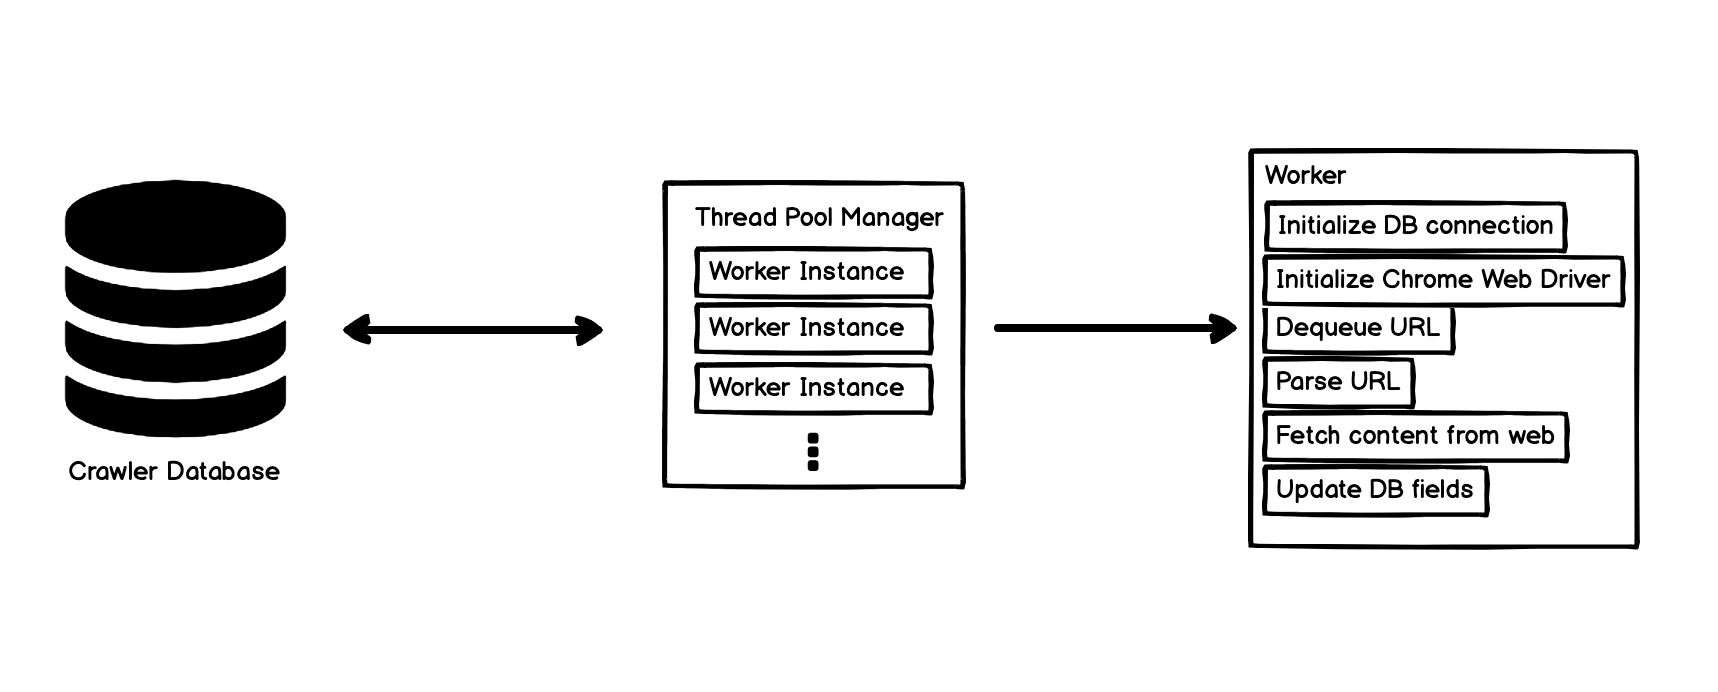
\includegraphics[scale=0.2]{flow_chart.png}
\subsubsection{Dequeue\_url}
is called on each worker and contains a while loop that terminates only when there are no more found urls to visit. Each worker gets a \textit{retry\_count} value of 50 which indicates after how many failed attempts at accessing an empty frontier it will cease to run. After each failed attempt the counter is decremented and the worker is forced to sleep for 10 seconds. In the event of a successfully acquired result the corresponding page's status is changed to "IN PROGRESS" to indicate that it is being processed. Afterwards the worker calls \textit{parse\_url(url, is\_binary)} and gives it the url and boolean value whether or not the contents are binary. 

\subsubsection{Parse\_url}
takes as arguments the url in a \textit{string} format and a boolean indicating if the url is binary or not. The url is converted into a canonical form and a number of different if statements are ran.
\begin{itemize}
\item If the url contents are binary just the site id is fetched with the function \textit{site\_id\_for\_domain}.
\item Alternatively the function \textit{parse\_robots} is executed which returns a site id and a \textit{robots\_parser} object.
\end{itemize}
Afterwards the \textit{robots\_parser} object is called and if it exists we check the desired crawl delay and make the worker sleep for as many seconds as it orders us to. If no such delay exists or we haven't managed to initialise the object we decided to implement a default 4 second delay before continuing. After the crawl delay is over the function \textit{fetch\_url} is called with the url, site id, the information if the contents are binary and the \textit{robot\_parser} object as arguments.

\subsubsection{Parse\_robots}
takes as it's argument a string of the desired url. It acquires the domain name of the url and tries to get the contents of the robots file if it already exists in the database. 
\begin{itemize}
\item If the contents are already stored it initialises it to a parser object and returns it along with the site id previously obtained from the database. 
\item Alternatively a request is made to the url of "robots.txt" and the returned content is then used to initialise a new robots parser object.
\end{itemize}
The chosen automatic robots parser does not do anything with the sitemap url as this is merely an extension of the "robots.txt" standard therefore we proceeded to parse it manually if this is our first time encountering this robots file. Using an xml parser we go through the contents of the sitemap and make the appropriate checks to determine if it is a valid government url. If the checks are successful we add the sitemap links to the frontier.


\subsubsection{Fetch\_url}
takes as it's arguments a url string representing the url of the site to be fetched, it's  \textit{id}, a boolean value is\_binary and the appropriate robots file parser. Afterwards a request is sent to the url which depending on the outcome can raise an exception or not. If no exception is raised a series of if statements handle which type of response we're dealing with. 
\begin{itemize}
  \item We check if the url contains a file that we can download. This is done with our \textit{should\_download\_and\_save\_file(url)} function. Alternatively we check the headers of the response if the file is of type \textit{msword}, \textit{powerpoint}, \textit{wordprocessingml.document} or \textit{presentationml.presentation}. In this case the \textit{save\_file} function is called with the url and response as arguments.
  \item If the boolean value (\textit{is\_binary}) is true or if the content type is \textit{image} the \textit{save\_image} function is ran with the url and response as arguments.
  \item If the response is of type \textit{text\textbackslash html} we attempt to render the page with the Selenium library. Since we have not figured out a practical way to make the library process already received responses we have to send another response to the url with the same library which then gets stored and the function \textit{parse\_page\_content(site\_id, url, status\_code, datetime.datetime.now(), robots)} is ran. If we get an error while rendering we update the status of the page in our database to 500 as most likely the site does not allow us to render it with Selenium.
  \item If the content type is something else the url data entry is updated in the database and page type value set to "UNKNOWN".
\end{itemize}
If our original request returned an error we get it's id from the database and update it's status to unreachable (404).

\subsubsection{Parse\_page\_content}
takes as arguments the id of the site, it's url, the status code and the time of last access. It acquires the page source and makes a hash out of it and tries to find an existing page id if such a page is already in the database via the function \textit{page\_for\_url(url)}. Afterwards it attempts to locate a duplicate page id with the function \textit{page\_for\_hash(hashed)} by using the hash of the page contents. 
\begin{itemize}
  \item If a duplicate id is found with the hash and if the url already exists in our database we simply update our existing page entry with information about the duplicate.
  \item If a duplicate id is found with the hash but if the url does not exist in our database we insert a new duplicate entry with information about the duplicate.
  \item If no duplicate is found with the hash but if the url already exists in our database we simply update our existing page entry.
  \item If no duplicate is found with the hash and no url already exists in our database we insert a new page entry into the database.
\end{itemize}
After these initial steps we begin the process of parsing the page.
\begin{itemize}
\item Using the BeautifulSoup library we get all the tags that contain the attribute "href" and check if they contain a valid government URL that hasn't already been visited. In such a case we add it to the frontier and update the pages status in the database.
\item Images are collected in a similar fashion by searching for the \textit{img} tag with BeautifulSoup. We then check if the links are valid and have not already been visited. In such a case we add them to the frontier however there have been cases when the links were invalid however the files could still be obtained by turning the links into their canonical form. A special few if statements are added at the end to handle such cases.
\end{itemize}

\section{Database}
Our database scheme remains the same as instructed with a few minor additions and upgrades:
\begin{itemize}
\item The page table now contains an extra \textit{hash} field with the value of the hash of the page contents.
\item The page table now contains an extra \textit{duplicate\_page\_id} field which contains the \textit{page\_id} of the first page seen with the same contents (the so called "original" page) of the given page entry. If a page does not have any duplicates this field is set to -1.
\item We've added two new page type codes. "IN PROGRESS" which lets our threads know that the given site is already being processed and "UNKNOWN" which signifies that the page is of an unknown type (not img, pdf or other).

\end{itemize}
\section{Crawling statistics}
network + general stats
\section{Conclusion}

 \bibliographystyle{apacite}
 
 \bibliography{references}


\end{document}
